\documentclass[11pt]{article}

% Use wide margins, but not quite so wide as fullpage.sty
\marginparwidth 0.5in 
\oddsidemargin 0.25in 
\evensidemargin 0.25in 
\marginparsep 0.25in
\topmargin 0.25in 
\textwidth 6in \textheight 8 in
% That's about enough definitions

% multirow allows you to combine rows in columns
\usepackage{multirow}
% tabularx allows manual tweaking of column width
\usepackage{tabularx}
% longtable does better format for tables that span pages
\usepackage{longtable}
\usepackage{graphicx}
\usepackage{hyperref}

\begin{document}

% this is an alternate method of creating a title
\hfill\vbox{\hbox{Team 13}
      \hbox{Huang, Jonathan}
      \hbox{Hoffman, Oliver}}\par

\bigskip
\centerline{\Large\bf CS5356: Homework 0}\par
\bigskip

\section{Team Members}
The members of the team are Jonathan Huang and Oliver Hoffman. We have been giving the GitHub Repo corresponding to Team 13 (\url{https://github.com/Cornell-CS5356-Fall2014/Team-13}).

\section{LAMP Stack}
A dummy PHP web page running on the LAMP stack can be found at \url{54.165.109.181}.

\section{Android Environment}
Screenshots to our Hello World test app with our team members' names are as follows:

\begin{figure}[h]
\centering
  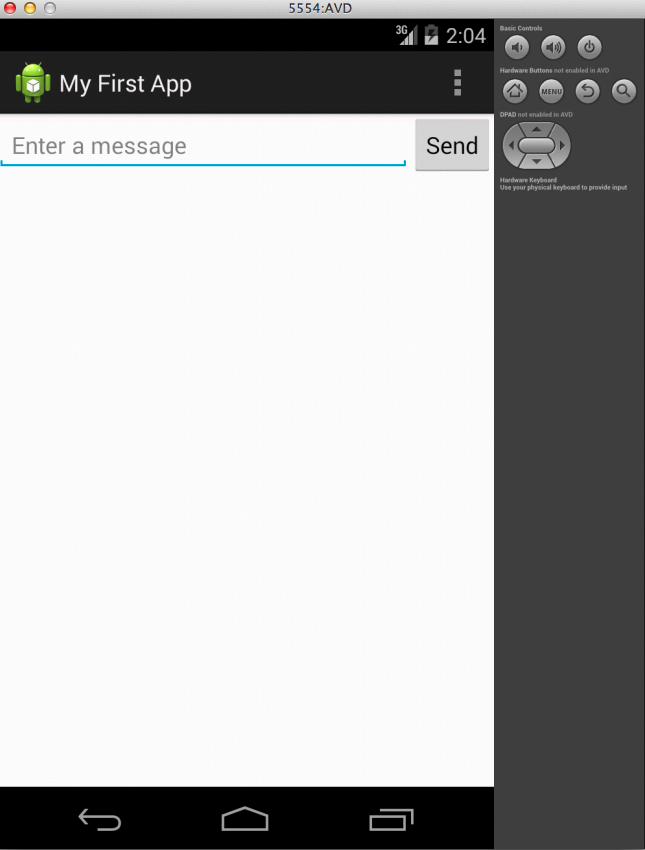
\includegraphics[scale=0.25]{home.png}
  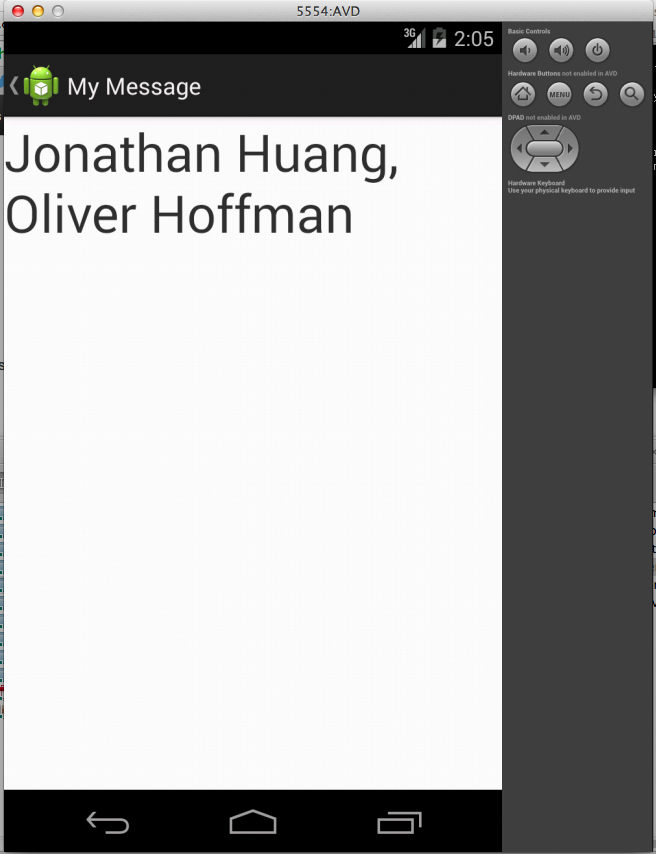
\includegraphics[scale=0.25]{names.png}
\end{figure}

\end{document}
